\documentclass[letterpaper, 10 pt, conference]{ieeeconf}  %
\IEEEoverridecommandlockouts                              % 
\overrideIEEEmargins                                      % 
\title{\LARGE \bf
A Model-based approach for testing\\intelligent transportation applications
}

\usepackage{bhadani_conf}

\graphicspath{ {figures/} }

\author{Rahul Bhadani$^{1}$, Matt Bunting$^{1}$ and Jonathan Sprinkle$^{1}$% <-this % stops a space
\thanks{*This work was supported by the National Science Foundation under award 1521617. \url{http://catvehicle.github.io}}% <-this % stops a space
\thanks{$^{1}$Rahul Bhadani, Matt Bunting and Jonathan Sprinkle are  with Department of Electrical \& Computer Engineering,
       The University of Arizona, 1230 E Speedway Blvd, Tucson 85719, Arizona, USA
        {Email: \sl\footnotesize \{rahulbhadani, mosfet, sprinkjm\}.email.arizona.edu}}%
}


\def\BibTeX{{\rm B\kern-.05em{\sc i\kern-.025em b}\kern-.08em
 T\kern-.1667em\lower.7ex\hbox{E}\kern-.125emX}}
 
 
 
\newcommand{\comment}[2][Comment]{\emph{{\marginpar{\color{blue}{\textsc{#1}}}}\textcolor{red}{#2}}\xspace}%
 
 
\begin{document}



\maketitle
\thispagestyle{empty}
\pagestyle{empty}



%%%%%%%%%%%%%%%%%%%%%%%%%%%%%%%%%%%%%%%%%%%%%%%%%%%%%%%%%%%%%%%%%%%%%%%%%%%%%%%%
\begin{abstract}
Please write some abstract here.

\end{abstract}


%%%%%%%%%%%%%%%%%%%%%%%%%%%%%%%%%%%%%%%%%%%%%%%%%%%%%%%%%%%%%%%%%%%%%%%%%%%%%%%%
\section{Introduction}
\label{sec:intro}
This is your introduction

\section{Background}
\label{sec:background}
Some background

\section{Model-Based Design}
\label{sec:mbd}
The vehicle model design is split into two parts: i) vehicle body or frame, and ii) chassis. We will discuss our approach for designing a realistic model to imitate a realistic scenario.

\subsection{Designing Robots with ROS}


 \begin{figure}[htbp]
    \centering
    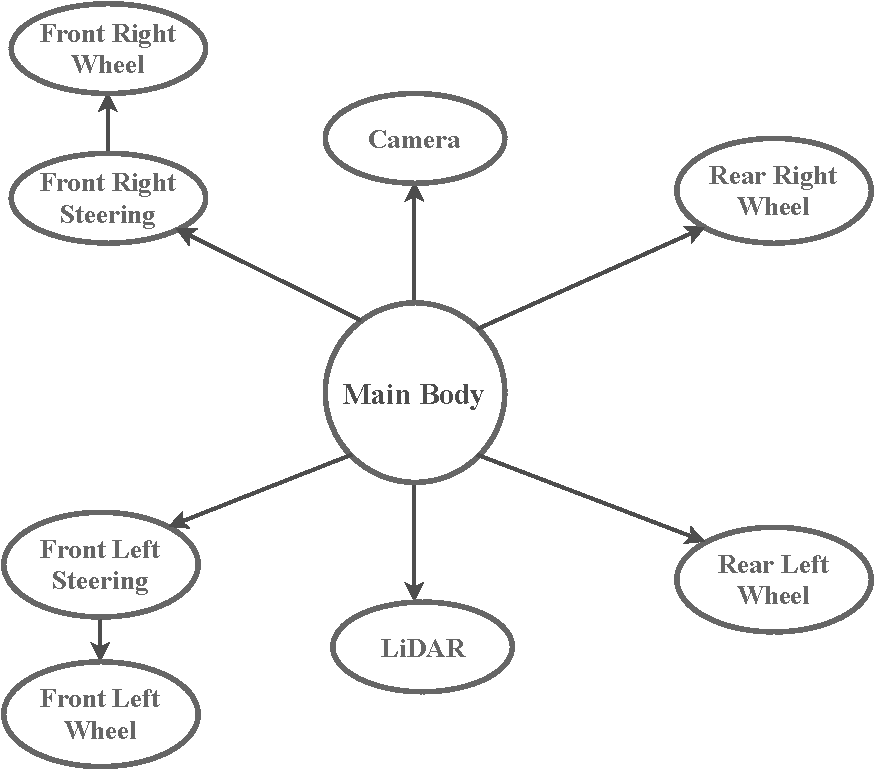
\includegraphics[angle=0,origin=c,trim={0.0cm 0.0cm 0.0cm 0.0cm},clip,width=1.0\linewidth]{urdfstruct.pdf}
    \caption{A graph structure of CAT Vehicle model.}
    \label{fig:urdfstruct}
    \end{figure}
    

\spliteq{
\label{eq:volume integrals}
\int_V p(x, y, z)dV
}

\begin{equation}
\label{eq:ex1}
	\begin{split}
	y = \pdv{(x^2 + e^x + \sin(x))}{x} + \pdv{x^5}{x} + \pdv{}{x}\cos x  + \log_2 x 
	\end{split}
\end{equation}

\begin{equation}
\label{eq:ex2}
A = \m{1 & 2 \\ 3 & 4}
\end{equation}

I am refering to Equation \eqref{eq:ex1} and \eqref{eq:ex2}.



\spliteq{
I_{xx} & = 347.195805 kg/m^2 \quad I_{xy} = -11.4914985 kg/m^2\\
I_{xz} & = 18.5070628 kg/m^2 \quad I_{yy} = 2330.10026 kg/m^2\\
I_{yz} & = 3.97814264 kg/m^2 \quad I_{zz} = 2529.41827kg/m^2
}

\subsection{Create Parts of Robots}
\label{sec:parts}
This where you define parts of robots

\section{Enabling Model-based design}
\label{sec:enablebd}



\section{Experiments and Results}
\label{sec:experiments}

Describe your experiment and results.

    
   
\section{Conclusion and Future Works}
\label{sec:conclusion}
What is the take home message from your research and how community benefited from it? Is there any shortcomings of this projects? Any limitation in the result you got? 
How will solve them in future? What are the possible extension and application of the current work? What would you like to do in the future?


\section*{ACKNOWLEDGMENT}
Support for this project was provided by the National Science Foundation and the Air Force Office of Scientific Research under awards 1659428.

\bibliographystyle{IEEEtran}
\bibliography{biblio}

\end{document}
